%\title{Overleaf Memo Template}
% Using the texMemo package by Rob Oakes
\documentclass[a4paper,11pt]{texMemo}
\usepackage[english]{babel}
\usepackage{graphicx, lipsum}

%% Edit the header section here. To include your
%% own logo, upload a file via the files menu.
\memosubject{Manuscript Revisions for \emph{Political Science Research and Methods}}
\memoto{PSRM-OA-2019-0085}
\memofrom{Complex Dependence in Foreign Direct Investment: Network Theory and Empirical Analysis}
\memodate{\today}


\begin{document}
\maketitle

\noindent We thank the editors for the opportunity to revise and resubmit our manuscript. In this memo
we have separated the editor's and reviewers' comments into separate criticisms and
suggestions. Under each comment, we describe how we have revised the manuscript in
response to the feedback provided. We generally agree with the criticisms offered, and think
that our manuscript has improved substantially as a result of incorporating this feedback. We note that, after trimming the original text, the additions that we have made in response to the reviewers have increased the word count by approximately 1,000. We think the material we have included in the manuscript is important to communicating our core contributions, but would be happy to move some of the content to the online appendix if necessary.


\section*{Editor}

\noindent \textbf{E1:} \emph{Both reviewers would like to see a more developed justification for the use of count ERGMs. R1 wants to know why the count ERGM is preferable to "spatial" models with exogenous connectivity matrices. Perhaps the most relevant model in this tradition is the dyadic model in Neumayer and Plümper, International Organization, Vol. 64, No. 1 (Winter 2010), pp. 145-166. With directed dyads, this model can handle reciprocity and transitivity. If the spatial lag is time lagged, one could model zero-inflation in a selection framework. R2 suggests that Hoff's AMEN model for networks can be easily amended to handle zero-inflation. R2 would also like to see some mention of Ward, Ahlquist and Rozenas.}\\

\noindent \textbf{Addressed:} These are all great points, and we realize that our treatment of existing modeling approaches was overly narrow in the initial submission. We extended our discussion of alternative approaches to note that three existing models---GERGM, AMEN, and N/P spatial, could all be used for dyadic FDI if they were extended to capture zero inflation. We note that developing such an extension would be beyond the scope of the current paper. Especially given that R1 is calling for additional substantive/theoretical discussion, we do not have sufficient space to add a substantial methods development objective to this paper. \\

\noindent \textbf{E2:} \emph{Both reviewers would like to see you address more of the literature on FDI. R1 points out that there's a literature on structural dependence across countries that goes back to Coughlin and Segev and includes several papers by Blonigen and Egger.} \\

\noindent \textbf{Addressed:} R1 spotted a blindspot in our coverage of dependence in the FDI literature. Though the work that we found is all monadic, it is still relevant to the study of dependence in FDI. We have added references to this literature, and note that we are building on it through the analysis of network forms of dependence. In particular, we added footnote 1 and the discussion on pp. 5--6.  \\

\noindent \textbf{E3:} \emph{R2 notes the research on PTAs and FDI and, based on the findings in this literature, would like you to control for trade agreements as well as BITs in your analysis}.\\

\noindent \textbf{Addressed:} We have added a PTA depth variable to all models and kept BITs in the updated models as well. We respond in more detail in R2.1\\

\noindent \textbf{E4:} \emph{R1 notes that your explanations for the two network effects seem to be rooted in different theoretical traditions. Reciprocity is older idea that is tied to market expansion while transitivity is rooted in the logic of global production chains.} \\

\noindent \textbf{Addressed:}  %TODO (Boliang), what  do we want to say about this?
In the earlier version, we built the reciprocity argument on two mechanisms: information diffusion and rivalrious expansion. In our revised version, we made the diffuse information mechanism the primary explanation. We also linked the diffusion mechanism to the global production networks, making the reciprocity and transitivity arguments more coherent. We believe that the information diffusion mechanism applies to both North-North and North-South dyads. In addition, we make the rivalrous expansion mechanism secondary. Reciprocal FDI resulting from MNCs' oligopolistic expansion strategy is predominately market seeking, which is more common among developed countries. \\

\noindent \textbf{E5:} \emph{R1 suspects that reciprocity may only apply to North-North dyads. (This seems to be borne out in Appendix F. ) I think it would be fruitful to explore these connections. Is reciprocity important for understanding North-North FDI and transitivity critical to understanding investment within mixed, North-South dyads that is driven by the multi-nationalization of production?}\\

\noindent \textbf{Addressed:} We added theoretical expectations regarding different reciprocity. Although we have witnessed a surge of FDI from developing countries since the early 2000s, MNCs from developing countries are still smaller and less competitive compared to their counterparts in developed countries and thus less likely to reciprocate. We expect reciprocity to be conditional. Our new empirical model explicitly accounts for the conditional reciprocity effects. We updated the \texttt{ergm} software package in R---a package version that we will distribute with our replication materials---to condition the reciprocity effect on a dyadic covariate. We find that reciprocity is positive, and stronger within dyads that include to OECD member countries, but that reciprocity among pairs of countries that include at least one non-OECD member is increasing over time.

Unfortunately, we are not able to address conditional transitivity in the current count ERGM model. We added a discussion of limitation in the conclusion. We expect transitivity to be stronger within mixed North-South dyads if FDI driven by global production networks is mainly vertical. The technical feature of transitivity calculation that makes calculating conditional transitivity much expensive than calculating conditional reciprocity is that the subgraph components (i.e., triples of nodes) cannot be separated into different types by partitioning the network adjacency matrix. For conditional reciprocity, the network adjacency matrix is partitioned prior to the enumeration of individual subgraph components. For calculating conditional transitivity, the full set of triples must be indexed in order to calculate dependence effects. Estimating conditional transitivity effects in a timely manner requires complex algorithmic extensions that are beyond the scope of our project.  \\

\noindent \textbf{E6:} \emph{R1 sees your findings with respect to political institutions as potentially important. Looking at Table 1, it seems like analyses that don't account for network effects tend to overstate the importance of both economic size and political institutions. Do we inflate the importance of these factors because there's so much reciprocal investment among the rich democracies?}\\

\noindent \textbf{Addressed:} In our revised manuscript, we have made three changes to the model specification: (1) added new covariates (PTA depth and OECD dummy); (2) slightly different DV rounding to reduce the effect of variable transformation; (3) accounted for conditional reciprocity. Our new results show that polity scores in destination countries are not a significant predictor of inward FDI in most years except for 2010--2012. The results suggest that the effect of democracy might be inflated in conventional models and in a model without actor heterogeneity (e.g., most reciprocal FDI happens among the rich democracies). This also seems to be the case for economic size. However, we also make a caveat that our operationalization of the DV is different from most existing studies that focus on net FDI inflows, which may lead to the discrepancy. Further, we note that future research is needed to understand the advantages and disadvantages of democratic institutions for different investors.\\

\noindent \textbf{E7:} \emph{R2 has a number of reasonable requests for the appendix: more on the estimation process; how is the multiple imputation handled; detailed GOF statistics.}\\

\noindent \textbf{Addressed:} We have removed the multiple imputation models from the Appendix, and added visualization of GOF statistics in the main draft. We respond to these points more in R2.6 and R2.8\\


\section*{Reviewer: 1}

\textbf{R1.1:} \emph{I completely agree with their primary criticism of the FDI literature: structural dependence across countries is a real problem in assessing any determinants of foreign direct investment.This paper is not the first to make that point; in fact spatial models FDI date back at least to Coughlin and Segev (2000), and perhaps earlier. In economics, Bruce Blonigen and Peter Egger have both investigated this topic with co-authors. But the real question for this paper is how to contribute to the political economy literature. The authors highlight several contributions in the paper, but I'm not sure that any fully succeeds in this version... Contribution number one is incorporating third-party effects on FDI. But are these network methods the best way to do that? On page 16, the authors suggest some other NETWORK estimators that might be appropriate, but they do not offer much evidence that network methods are better than other spatial methods. I have some skepticism on this point, given that the authors must use a count model to estimate the correlates of foreign direct investment stock. They choose their dependent variable based on the model's needs, and their hypotheses are limited to 'canonical forms of network structure' (p. 21). Surely other spatial models are better equipped to test multiple types of spatial effects that allow for more sophisticated spatial effects. For example, the network model cannot discriminate between third-country effects that are positive because FDI happens between countries A and B and where it is negative because of that transaction. An auto parts plant in Czech Republic may mean more FDI for Hungary, but a toothpaste plant may mean less because it uses one plant to serve all eastern countries in the European Union. In other words, it depends on the logic of the investment, but global supply chains have complex effects, not just increasing FDI everywhere. In fact, it remains highly concentrated... the authors exhibit a deep knowledge of the foreign direct investment literature, but they use that literature to justify the limited hypotheses that can be tested in network models. In its current form, the paper finesses this point, but it seems that in the end the authors are relatively honest, noting their 'network theory of FDI that includes reciprocity and transitivity as the core structural dependencies' (p. 29). If the others can make the case why network models have unique advantages, then why be indirect about the limitations of those theories. Be honest about what can be tested and what cannot. Crucial here is justifying how network models are better than other spatial models.}\\

\noindent \textbf{Addressed:}  We thank R1 for pointing us to the highly relevant literature on spatial dependence in FDI. We have incorporated a discussion of this work, and noted that we are building on this research in theorizing about and estimating other forms of dependence---network dependencies. It is not entirely clear to us based on this comment what R1 has in mind in terms of ``more sophisticated spatial effects'', but we agree, and now more openly acknowledge in the paper, that we are constrained by the software in terms of what forms of dependence can be modeled. We also note that the ERGM can theoretically represent any form of dependence---a result that has been noted several times with reference to the Hammersley-Clifford Theorem. This would include any form of spatial dependence that could be conceptualized. The pragmatic challenge, of course, is theorizing and implementing the structural terms that reflect multiple forms of dependence.  \\


\noindent \textbf{R1.2:} \emph{Contribution number two is yet another take on political institutions and FDI. This may appear to be settled given the extensive meta-analysis in Li, Owen, and Mitchell (2018, henceforth LOM), but few if any of the papers they review account for third-party FDI effects. As such, this paper can reignite that literature, as all other papers can be critiqued as misspecified. Additionally, LOM find that the debate over whether democracy attracts FDI is governed by the choice of measure, but FDI stocks are not as commonly used as flows and therefore may show different results. Any finding here must deal with the critique by Arel-Bundock (2017) that political institutions are just not very important for FDI.}\\

\noindent \textbf{Addressed:} We thank R1 for the excellent comment. As mentioned in our response to E6, we have made three changes to our model specification. The new results suggest that the coefficient of destinations' democracy is not significant in most years except for 2010--2012. We made two points on pp. xx. First, our DV---FDI stocks---is different from most existing studies that use net FDI inflows, which may lead to the discrepancy. Second, our results could suggest that the effect of democracy in conventional models is overestimated. We have made reference to Arel-Bundock (2017). \\


\noindent \textbf{R1.3:} \emph{Contribution number three is the focus on expansion of global supply chains, given the unique timeframe of the data. The relationship between FDI and trade may therefore be unique to this time period, and care should be taken regarding generalization of the results. Again the network setup limits the analysis of panel data to either pooled or multiple cross-sections, but the authors do as well as can be expected with these limitations. Strangely, the first hypothesis is justified with older motivations for MNCs (who saturate domestic markets and must look abroad for profits) rather than theories that are more attuned to cross-border supply chains. Their logic seems appropriate for rich country pairs, but much less so for North-South dyads. I expect the results do not hold for non-OECD countries.}\\

\noindent \textbf{Addressed:}  We agree with R1. Accordingly, we have added a discussion on the limitation of our study on pp. xx. Given that our data covers the period of 2001--2012 only, we are cautious about generalizing the results to earlier periods. We also agree that reciprocity is more prevalent for North-North dyads. Our new model specification accounts for conditional reciprocity and our results indeed show that reciprocity is stronger among pairs of OECD countries than pairs of non-OECD countries and mixed pairs. Although reciprocal FDI is more common among North-North dyads, we also find significant reciprocity in recent years among North-South dyads. This is consistent with the fact that developing-country firms have become increasingly important global investors recently. To make our theoretical arguments more coherent, we have made the information diffusion mechanism the primary explanation for reciprocity and linked it to the global production networks. We believe this is a more general mechanism that applies to both North-South and North-North dyads. In addition, we have made the rivalrious expansion mechanism secondary, which is more common for North-North dyads. See also our responses to E5 and E6.  \\


\noindent \textbf{R1.4:} \emph{...the dependent variable is imperfect in ways that are not addressed. UNCTAD has done great work on this data set, and I'm glad the authors are making use of it. Furthermore, I like that they use a lagged dependent variable, which might initially make the setup seem similar to a model of FDI flows because it looks for variation in the one year changes of stocks. FDI stocks, however, can vary from year to year for multiple reasons, including both new flows and revaluation. For example, the book value of a factory may deteriorate from one year to the next due to the depreciation of capital assets. To the extent that these depreciation's are reflected in the FDI stocks measure, it is more than just a representation of flows. Perhaps controlling for inflation would solve this problem, but I am not optimistic of any real solution. Furthermore, the measure still aggregates data at the country level, although the decision-makers are firms. These are important limitation of the data, and should be mentioned in the text.}\\

\noindent \textbf{Addressed:} We agree with R1 that the book value of FDI stocks can change due to factors other than new flows. Following R1's suggestion, we have run a robustness check by controlling for inflation. We have also controlled for exchange rates to further address the issue. Our main results remain the same. In addition, we have added a discussion of the limitation of the data on pp. xx, acknowledging that our aggregate FDI measure is at the country level, though our theory is built on firm-level investment decisions. It would be fruitful to explore firm-level investment networks in future research.  \\

\section*{Reviewer: 2}


\noindent \textbf{R2.1:} \emph{One simple request that I have is that the authors account for the effect that PTAs may have on FDI. Though PTAs are often thought of as simply means to ensure reciprocal market access vis a vis adjustment of tariffs and related border measures, more recent PTAs contain provisions that cover a wide array of non-tariff measures such as rules on investment and intellectual property rights protection. The DESTA database provides a very useful way to account for these types of deep PTAs and I'd be interested in seeing whether or not that parameter accounts for some of the clusters the authors are picking up through their transitivity term. The relationship between PTAs and FDI is not uncommon in the literature, for example, see Buthe \& Milner (2008), Medvedev (2012), and Osnago et al. (2016).}\\

\noindent \textbf{Addressed:} While the literature that we cited and R2 mentions uses a count variable for PTAs, we agree with R2 that the DESTA database is very useful to control for differences between PTAs. We opted to use the latent space measure of PTA depth from DESTA  in the updated models and made sure that the variable was not too highly correlated with the BIT binary variable as ERGMs are sensitive to multicollinearity. The transitivity coefficient is smaller in the updated models, but remains positive and significant. \\

\noindent \textbf{R2.2:} \emph{I was surprised to not see a term for actor heterogeneity in the model. I imagine this could manifest in the FDI network for a variety of reasons (beyond those accounted for by the already included covariates) as some countries are more active or reliant on FDI than others. It would be useful to at least see an Appendix item in which the authors include a term for actor heterogeneity in the model and present the results in a format similar to Table 1.}\\

\noindent \textbf{Addressed:} Please see our response to R2.8. \\

\noindent \textbf{R2.3:} \emph{In general, more detail should be provided at least in an appendix about the estimation process for the count ERGM. I'm guessing the authors are using the model from Krivitsky (2012), which provides a way to estimate ERGM on valued networks and specifically dispersed count dependent variables but it would be useful if this was made clearer in the manuscript, especially since this has been submitted in a methods journal.}\\

\noindent \textbf{Addressed:} We added a paragraph to Section 3.2.1 in which we discuss the specific form of the count ERGM we use---the Poisson ERGM from Krivitsky (2012), and discuss how the parameters are estimated. \\

\noindent \textbf{R2.4:} \emph{On page 14, the authors note that the count ERGM is "the only network model that can currently be used to model weighted data with zero-inflation". This is not correct as the Ward, Ahlquist, and Rozenas (2013) piece introduced a latent space model for trade data to account for the excess of non-trading dyads via a mixture approach. I understand that the authors are interesting in estimating substantive effects for network terms such as transitivity, which cannot be done via a latent space or factor approach, but the quoted text should be corrected. Additionally, extending Hoff's AMEN framework to handling dispersed count processes is also a trivial task.}\\

\noindent \textbf{Addressed:} Please see our response to E1. We have expanded our discussion to engage these approaches, and extensions thereof, as alternative methods.\\

\noindent \textbf{R2.5:} \emph{Additionally, the choice to model FDI as a count process is something that I at least have not often encountered in the FDI literature. I understand that extending GERGM in a way to handle the excess of zeros is not straightforward, but it would be helpful if the authors provided some grounding for their choice beyond noting that an ERGM for a continuous dependent variable with an excess of zeros does not exist.}\\

\noindent \textbf{Addressed:} Our only reason for converting the log of FDI to a count and using the count ERGM is, ``that an ERGM for a continuous dependent variable with an excess of zeros does not exist.'' However, in the revised paper and supporting information we have done more to investigate the empirical consequences of rounding FDI. If we used the un-rounded version of log-FDI as the outcome variable, we would be following a very common approach in the literature. Where we depart from the literature is in rounding the log-FDI values. In the supporting information we now present an assessment of whether rounding to create a count significantly changes the associations between any of the dyadic covariates and FDI. We present tables of the correlations between independent variables and FDI, as well as hypothesis tests of the differences between these correlations. The correlations are all very similar, and rounding does not result in a single difference that is significant at conventional levels. We see this as evidence that rounding logged FDI does not significantly change the structure of associations in which FDI is embedded. \\

\noindent \textbf{R2.6:} \emph{In terms of dealing with missing data, the authors have effectively applied a number of robustness checks. However, the robustness check I was most interested in was Section D of the Appendix, in which they imputed via Amelia. Specifically, how was the imputation and estimation process done, were multiple imputed datasets generated and then count ERGMs run on each imputed dataset? How were the parameter estimates results from each of the ERGM-imputed datasets combined? Was it simply a matter of employing Rubin's rules?}\\

\noindent \textbf{Addressed:} We thank R2 for catching the lack of discussion regarding the multiple imputation robustness check, given it is not commonly used for ERGMs. For the imputations, we used the dataset that included all covariates and imputed the column for the original FDI stock values and then transformed the data for the models. We used ten imputations, modeled each imputed dataset and then combined the parameter estimates using standard Rubin's rules. However, in the updated version of the paper, we have decided to drop the multiple imputation robustness check, and include only the check in which we subset to countries with more complete data. We have two reasons for dropping the MI check. First, upon closer review of the imputed datasets, we found the distributions of bilateral FDI to be highly unrealistic, resulting in sums of bilateral FDI that far exceed countries' total reported FDI. Shown in Figure \ref{fig:MIcheck}, imputed values have a much higher average value and a lower variance than actual reported totals. This results from the fact that the reported FDI flows tend to be large, and their scale feeds through to the imputed values in the MI. Second, upon closer review of the literature in IPE that uses dyadic data, we recognized how common it is to subset to sets of countries for which consistent data is available. Thus, we see the robustness check based on subsetting countries as sufficient for our analysis.\\

\begin{figure}[!h]
\centering
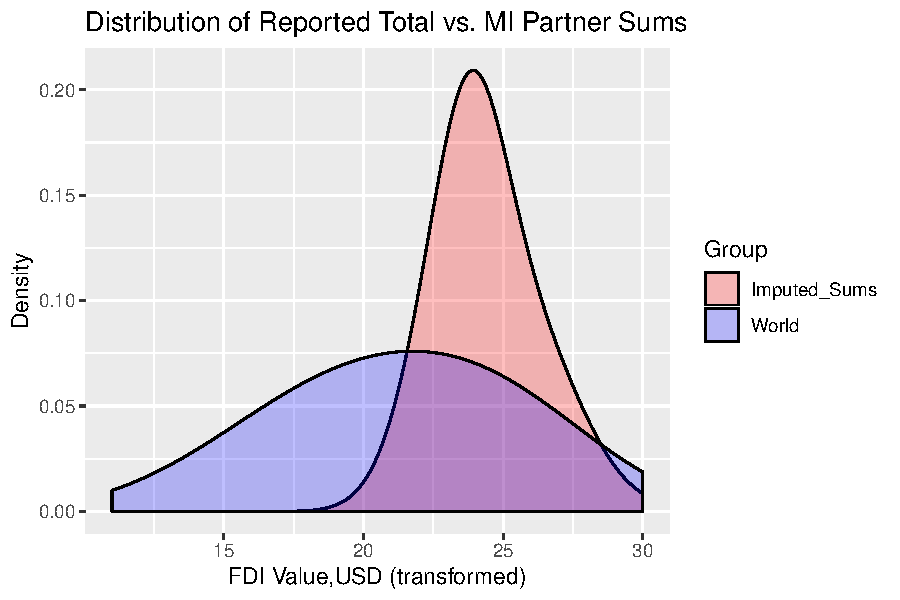
\includegraphics[scale=.75, clip=true, trim=0cm 0cm 0cm .8cm]{check_MIsums_logged.pdf} \vspace{-.5cm}
\caption{\label{fig:MIcheck} Density plots of reported FDI yearly totals for countries from world  and average summed totals after parametric multiple imputation. Transformation of FDI values follows the same steps as in the paper.}
\end{figure}




\noindent \textbf{R2.7:} \emph{For Figure 2, I'd be interested in seeing the results broken out by year. Additionally, I think that a corresponding yearly figure for transitivity is useful and necessary. Of course, figure 3 is helpful in terms of showing that the transitivity and reciprocity parameters are significant but I would like to know how far away a model without network terms is in accounting for transitivity especially after the authors have accounted for PTAs. My guess is that the network model will still outperform the canonical approach, and this will strengthen the key contribution being made by the authors.}\\

\noindent \textbf{Addressed:} Please see our response to R2.8.  \\

\noindent \textbf{R2.8:} \emph{Whenever I see an ERGM I also always want to see detailed GOF statistics. Some tests of how well the authors' proposed model accounts for standard ERGM GOF diagnostics relative to a model without network dependence terms would be useful. I imagine the authors will just include these results in an Appendix but in my opinion they must be included so that we can be sure the ERGM is properly specified.}\\

\noindent \textbf{Addressed:}  This suggestion, combined with R2's comments regarding degree heterogeneity and extending fit comparisons across multiple years, is a very helpful line of discussion. We initially omitted extensive structural fit comparisons (as are common in papers using binary ERGMs), and opted to rely solely on BIC, due to the lack of standard structural fit measures for count ERGM. However, now that we have revisited this omission, and added a set of fit assessments using various statistics available in the literature, our paper provides an initial example of structural fit assessment with count ERGM.  The count ERGM provides a reasonable structural fit to weighted measures of reciprocity, transitivity, and in-degree heterogeneity, but not to out-degree heterogeneity. We note that the development of less degeneracy-prone specifications for degree distribution is an important direction for future methods research. To assure that our main results regarding reciprocity and transitivity are robust to the use of a model that accounts for actor heterogeneity, in Appendix D we present estimates using AMEN (with un-transformed FDI stock and Gaussian-distributed edges). \\
\\

\end{document} 